\section{Observer-Muster}
\subsection{Problemstellung}
- Wetterstation liefert Daten (Luftdruck, Temperatur, etc.).
- Gefragt ist ein WetterDaten-Objekt. 
- Diverse Anzeigegeraete sollen in der Lage sein, sich die Daten vom WetterDaten-Objekt zu ziehen 
  und entsprechend darzustellen. Problematisch wird es, wenn verschiedene Anzeigegeraete nur 
  bestimmte Daten anzeigen sollen. 
- Besonderes Augenmerk bei dieser Aufgabe, die Daten sollen mit einem einzigen Aufruf 
  aktualisiert werden. 
- Wichtig: Es soll moeglich sein neue Anzeigeraete einzubinden. Hierbei soll der zus. Aufwand so 
  gering wie moeglich gehalten werden. 

\subsection{L"osung}
Observer-Muster (Grundsaetzliches Prinzip):
Man definiert ein Interface z.B. "Subjekt" das die Schnittstelle fuer das WetterDaten-Objekt 
angibt. Hierzu gehoeren die Methoden um einen Beobachter zu registrieren, zu entfernen oder 
diesen ueber die Aktualisierung der Daten zu informieren (bzw. ihm diese zukommen zu lassen). Die 
Idee beim Observer-Muster ist naemlich, dass ein Datenobjekt mit entsprechenden Feldern ein 
Attribut mit einer Liste von Beobachtern haelt die Zugriff auf die Felder besitzen. Dies kann 
mithilfe einer Uebergabe des Objektes geschehen oder aber mit einer tatsaechlichen Uebergabe von 
Parametern. Mit den Methoden zum Registrieren und Entfernen werden die Beobachter der Liste 
hinzugefuegt oder entfernt. Das WetterDaten-Objekt aus dem Bsp. implementiert jetzt dieses 
Interface. Anschliessend wird ein zweites Interface fuer die Beobachter (im Bsp. die 
verschiedenen Anzeige-Klassen) geschrieben. Die Beobachter informieren dieses jeweils und haben 
damit Zugriff auf eine Methode zum Aktualisieren der Werte. Hier koennen direkt die Parameter 
uebergeben werden, oder aber das Datenobjekt selbst (um mit Gettern die Daten zu uebermitteln). 

Observable-Muster aus java.util.Observable / Observer 
Es gibt bereits ein vorgefertigtes Observer-Muster in der Standardbibliothek util. Hier erbt das 
jeweilige Datenobjekt von der Superklasse Observable. Diese Klasse bringt bereits die Liste aus 
Beobachtern und weitere Methoden wie die setChanged() und notfyObservers() Methoden. Wichtig 
hierbei ist zu beachten, dass man erst die Beobachter benachrichtigen kann wenn setChanged 
aktiviert wurde. NotifyObservers() ist ausserdem ueberladen, denn es ist ist moeglich neben dem 
eigentlichen Datenobjekt (hier WetterDaten-Objekt) noch ein anderes zu uebergeben, welches z.B. 
weitere Werte enthalten kann. 
Zum genauen Aufbau siehe Code.

\paragraph{Nachteile der Standardbibliothek}
\begin{itemize}
\item Reihenfolge der Auswertung aendert sich -> Ungeeignet fuer Anwendungen wo dies von Bedeutung 
  sein sollte.
\item Observable ist eine Klasse und kein Interface -> Klasse kann daher keine andere Klasse 
  erweitern und schlecht wartbar sowie wiederverwendbar.
\item Observable schuetzt entscheidende Methoden -> z.B. setChanged(), kann daher auch nur von 
  erbenden Klassen aufgerufen werden.
\end{itemize}
  
Vorteile: Siehe AufgZuDenEntwurfsprinzipien.txt

\subsection{Erkl"arung des Musters}
\paragraph{Definition}
Das Observer-Muster definiert eine Eins-zu-viele-Abhaengigkeit zwischen Objekten in der Art, dass 
alle abhaengigen Objekte benachrichtigt werden, wenn sich der Zustand des einen Objekts aendert. 

\paragraph{Gutes Alltagsbeispiel} 
Zeitungsabonnementsdienst
\begin{itemize}
\item Man moechte Abonnent werden -> man wird auf die Liste der Abonennten gesetzt. 
\item Neue Ausgabe wird ausgegeben (aktualisiert) -> Alle Abonnementen der Liste werden benachrichtigt. 
\item Bei der Standardbibliothek utils ist bereits ein solches Muster vorgegeben mit dem es fuer die 
  Abonennten sogar moeglich ist sich jederzeit per Getter-Methoden die Daten zu ziehen ohne das 
  eine entsprechende Methode im Subjekt aufgerufen werden muss.
\item Auf Wunsch ist es ebenfalls moeglich wieder aus der Liste der Abonennten auszutreten. 
\end{itemize}

\paragraph{Punkt fuer Punkt Zusammenfassung (S. 74)}
\begin{itemize}
\item Das Observer-Musster definiert ein Eins-zu-viele-Verhaeltnis zwischen Objekten.
\item Subjekte oder, wie wir sie auch kennen, Observables aktualisieren Beobachter ueber eine 
  Schnittstelle.
\item Die Beobachter sind insofern locker angebunden, als das Bbservable ueber sie nichts anderes 
  weiss, als dass sie das Interface Observer implementiern. 
\item Sie koennen Daten aus dem Observable herausgeben oder herausziehen, wenn Sie das Muster 
  verwenden (wobei das Herausziehen als die "richtigere" Methode betrachtet wird). 
\item Verlassen Sie sich nicht auf eine bestimmte Reihenfolge der Benachrichtigung Ihrer Beobachter. 
\item Java besitzt eine Reihe von Implementierungen des Observer-Musters, einschliesslich des 
  allgemeinen java.util.Observable.
\item Nehmen Sie sich vor den Haken der Implementierung von java.util.Observable in Acht. (Siehe 
  Erklaerung Kap. 1).
\item Haben Sie keine Hemmungen, Ihre eigene Observable-Implementierung zu schreiben, wenn dies 
  erforderlich ist.
\item Swing macht wie andere GUI-Frameworks extensiven Gebrauch vom Observer-Muster.
\item Sie finden das Muster auch an vielen anderen Orteien einschliesslich JavaBeans und RMI. 
\end{itemize}

\subsection{Aufgabe zu den Entwurfsprinzipien}
\paragraph{Aufgabe zu den Entwurfsprinzipien}
Beschreiben Sie fuer jedes Entwurfsprinzip, wie das Observer-Muster das Prinzip umsetzt. 

\paragraph{Prinzipien}
\begin{enumerate}
\item Identifizieren Sie die Aspekte Ihrer Anwendung, die sich aendern koennen und trennen Sie sie 
   von denen, die konstant bleiben.
\item Programmieren Sie auf eine Schnittstelle, nicht auf eine Implementierung.
\item Ziehen Sie die Komposition der Vererbung vor.
\end{enumerate}

\paragraph{Eigene Erkl"arung}
\begin{enumerate}
\item Beobachter koennen sich aendern, werden daher zusammengefasst und ausgelagert.
\item Da die Beobachter lediglich ein Interface implementieren und keine Klasse erweitern, besteht 
   hier eine lose Bindung d.h. man Programmiert auf eine Schnittstelle.
\item Die beiden Parteien (Beobachter, Subjekt) implementieren jeweils nur ein Interface und 
   erweitern keine Superklasse.
\end{enumerate}
   
\paragraph{Erklaerungen aus dem Buch (S. 77)}
\begin{enumerate}
\item Das, was beim Observer-Muster variiert, ist der Zustand des Objekts und die Anzahl sowie die 
   Typen der Beobachter. Mit diesem Muster koennen Sie die Objekte variieren, die vom Zustand des 
   Objekts abhaengig sind, ohne das Subjekt veraendern zu muessen. Das nennt man verausschaen 
   handeln!
\item Subjekt und Beobachter nutzen beide Interfaces. Das Subjekt haelt Objekte nach, die das 
   Interface Observer implementieren, waehrend die Beobachter sich registrieren und vom 
   Subjekt-Interface benachrichtigt werden. Wie wir gesehen haben, haelt das die die Dinge 
   ordentlich und locker gebunden. 
\item Das Observer-Muster nutyt Komposition um eine beliebige Anzahl von Beobachtern mit ihren 
   Subjekten zu verbnden. Diese Beziehungen werden nicht durch irgendeine Art von 
   Vererbungshierachie implementiert. Nein sie werden zur Laufzeit durch Komposition eingerichtet!
\end{enumerate}

\begin{figure}
	\centering
	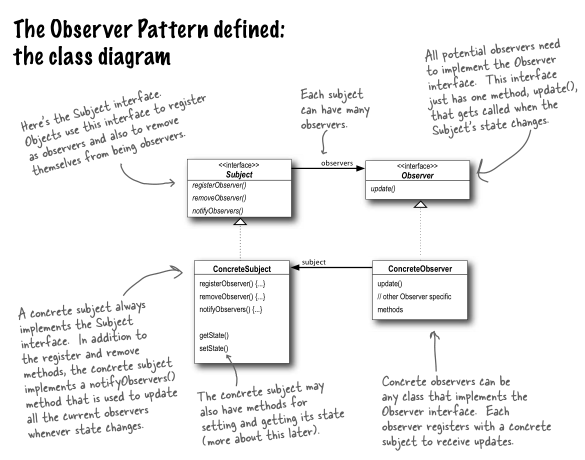
\includegraphics{observer/img/observerUML}
	\caption{UML-Darstellung des Observer-Musters}
	\label{fig:observerUML}
\end{figure}
